%\documentclass[letterpaper,twocolumn,10pt]{sig-alternate-10pt}
%\usepackage{epsfig,endnotes}
%\documentclass[letterpaper,twocolumn,10pt]{article}
%\usepackage{usenix,epsfig,endnotes}
%\documentclass[letterpaper,twocolumn]{hotnets16}
\documentclass[letterpaper,twocolumn]{hotnets17}
\usepackage{epsfig,endnotes}

%\usepackage{geometry}
%\geometry{top=1in}

\usepackage{mathptmx}	
\usepackage{amsmath}
\usepackage{amssymb}
\usepackage{amsfonts}
\usepackage{bbding}



\usepackage[font=bf]{caption}
\usepackage{quoting}
\usepackage{csquotes}
\SetBlockEnvironment{quoting}

\usepackage{subfig}
%\usepackage{subfigure}

\usepackage{multirow}
\usepackage[linesnumbered,noend,boxed]{algorithm2e}
\setlength{\textfloatsep}{0.2cm}

\newcommand{\subparagraph}{} 
\usepackage[usenames,dvipsnames]{color}

\usepackage[compact]{titlesec}

\usepackage{amsmath}
\usepackage{amsfonts}


\usepackage{times}

\usepackage{xspace}
\usepackage{epsfig} 
\usepackage{amsmath}
\usepackage[hyphens]{url}
\usepackage{amsfonts} 

\usepackage{booktabs}
\usepackage{multirow}
\usepackage{graphicx}
\usepackage[table,xcdraw]{xcolor}

\usepackage{listings}
\usepackage{fancyvrb}
\usepackage{mathrsfs}
\usepackage[bordercolor=white,backgroundcolor=gray!30,linecolor=black,colorinlistoftodos]{todonotes}
\VerbatimFootnotes

%\usepackage[hhmmsstime]{datetime}
\usepackage[12h=false]{scrtime}

\usepackage{tablefootnote}

\usepackage[normalem]{ulem}



%\setlength{\pdfpagewidth}{8.5in}
%\setlength{\pdfpageheight}{11in}

%\usepackage{mdframed}

\newtheorem{theo}{Insight}
\newenvironment{ftheo}
  {\begin{mdframed}\begin{theo}}
  {\end{theo}\end{mdframed}}

%\newcommand{\insightref}[1]{\textbf{Insight}\ref{#1}}
%\newcounter{insightlabel}
%\renewcommand{\theinsightlabel}{\textbf{I}}
%\newenvironment{insight}{
%\begin{list}{\textbf{Insight}\theinsightlabel:~}{\usecounter{insightlabel}\setlength{\labelwidth}{0pt}\setlength{\labelsep}{0pt}\setlength{\leftmargin}{0in}\noindent\rule{\linewidth}{1pt}\vspace{-9pt}\item \bf \em}}{\\[-7pt]\end{list}\vspace{-11pt}\noindent\rule{\linewidth}{1pt}}

%\newcommand{\insightref}[1]{\textbf{Insight }\ref{#1}}
\newcommand{\insightref}[1]{{Insight }\ref{#1}}
\newcounter{insightlabel}
\newcounter{insightnmbr}
%\renewcommand{\theinsightlabel}{\textbf{\theinsightnmbr}}
\renewcommand{\theinsightlabel}{{\theinsightnmbr}}
\newenvironment{insight}{
\vspace{-0.0cm}
\begin{list}{\textbf{Insight }\theinsightlabel:~}{\usecounter{insightlabel}\stepcounter{insightnmbr}\setlength{\labelwidth}{0pt}\setlength{\labelsep}{0pt}\setlength{\leftmargin}{0in}\noindent\rule{\linewidth}{1pt}\vspace{-10pt}\item \bf \em}}{\\[-7pt]\end{list}\vspace{-10pt}\noindent\rule{\linewidth}{1pt}}

%\newcommand{\impref}[1]{\textbf{Corollary 3.}\ref{#1}}
\newcommand{\impref}[1]{{Corollary 3.}\ref{#1}}
\newcounter{implabel}
\newcounter{impnmbr}
%\renewcommand{\theimplabel}{\textbf{\theimpnmbr}}
\renewcommand{\theimplabel}{{\theimpnmbr}}
\newenvironment{imp}{
\vspace{-0.0cm}
\begin{list}{\textbf{Corollary 3.}\theimplabel:~}{\usecounter{implabel}\stepcounter{impnmbr}\setlength{\labelwidth}{0pt}\setlength{\labelsep}{0pt}\setlength{\leftmargin}{0in}\noindent\rule{\linewidth}{1pt}\vspace{-9pt}\item \bf \em}}{\\[-7pt]\end{list}\vspace{-11pt}\noindent\rule{\linewidth}{1pt}}


\newcommand{\tightcaption}[1]{\vspace{-0.12cm}\caption{{\em #1}}\vspace{-0.13cm}}
%\newcommand{\tightsection}[1]{\vspace{-0.02in}\section{#1}\vspace{-0.03cm}}
%\newcommand{\tightsubsection}[1]{\vspace{-0.02in}\subsection{#1}\vspace{-0.03cm}}
\newcommand{\tightsection}[1]{\vspace{-0.08cm}\section{#1}\vspace{-0.08cm}}
\newcommand{\tightsubsection}[1]{\vspace{-0.08cm}\subsection{#1}\vspace{-0.08cm}}
%\newcommand{\tightsection}[1]{\vspace{-0.0cm}\section{#1}\vspace{-0.0cm}}
%\newcommand{\tightsubsection}[1]{\vspace{-0.0cm}\subsection{#1}\vspace{-0.0cm}}
\newcommand{\tightsubsubsection}[1]{\vspace{-0.01in}\subsubsection{#1}\vspace{-0.01cm}}

\newcommand{\eg}{{\it e.g.,}\xspace}
\newcommand{\ie}{{\it i.e.,}\xspace}

\newcommand{\comment}[1]{}
\newcounter{note}[section]
\renewcommand{\thenote}{\thesection.\arabic{note}}

\newcommand{\Section}{\S}

\usepackage{pifont}
\newcommand{\cmark}{\ding{51}}%
\newcommand{\xmark}{\ding{55}}%

\newcommand{\fillme}{{\bf XXX}~}

\newcommand{\dda}{{CFA}\xspace}
\newcommand{\system}{{\dda}\xspace}
\newcommand{\ControlPlane}{{global optimization system}\xspace}

%\newcommand{\name}{{TBD}\xspace}
\newcommand{\ddn}{{DDN}\xspace}

\newcommand{\mypara}[1]{\smallskip\noindent{\bf {#1}:}~}
\newcommand{\myparatight}[1]{\vspace{0.03cm}\noindent{\bf {#1}:}~}
\newcommand{\myparaq}[1]{\smallskip\noindent{\bf {#1}?}~}

\newcommand{\myparaittight}[1]{\smallskip\noindent{\emph {#1}:}~}
\newcommand{\question}[1]{\smallskip\noindent{\emph{Q:~#1}}\smallskip}
\newcommand{\myparaqtight}[1]{\smallskip\noindent{\bf {#1}}~}

\newcommand{\vyas}[1]{{\footnotesize\color{red}[VS: #1]}}
%\newcommand{\is}[1]{{\footnotesize\color{orange}[IS: #1]}}
%\newcommand{\jc}[1]{{\footnotesize\color{blue}[JC: #1]}}
%\newcommand{\xil}[1]{{\footnotesize\color{magenta}[XI: #1]}}
%\newcommand{\hm}[1]{{\footnotesize\color{Maroon}[HM: #1]}}
%\newcommand{\ai}[1]{{\footnotesize\color{Purple}[TODO: #1]}}

%\newcommand{\vyas}[1]{{\footnotesize\color{red}{}}}
\newcommand{\is}[1]{{\footnotesize\color{orange}{}}}
\newcommand{\jc}[1]{{\footnotesize\color{blue}{[JC: #1]}}}
\newcommand{\newjc}[1]{{\footnotesize\color{blue}}}
\newcommand{\xil}[1]{{\footnotesize\color{magenta}{}}}
\newcommand{\hm}[1]{{\footnotesize\color{Maroon}{}}}
\newcommand{\ai}[1]{{\footnotesize\color{Purple}{}}}

\newcommand{\camera}[1]{{\color{black}{#1}}\xspace}
%\newcommand{\cameraremove}[1]{{\color{blue}{\sout{#1}}}}
\newcommand{\cameraremove}[1]{{\color{black}{}}\xspace}
\newcommand{\vyascomment}[1]{{\color{red}{#1}}\xspace}
\newcommand{\vyasremove}[1]{{\color{red}{}}\xspace}

%\newcommand{\new}[1]{\color{purple}{#1} \color{black}}
\newcommand{\new}[1]{\color{black}{#1} \color{black}}
\newcommand{\old}[1]{{\color{black}{}}}

\newcommand{\name}{{SysName}\xspace}

%\newcommand{\seyed}[1]{{\footnotesize\color{blue}[SF: #1]}}
%\newcommand{\alig}[1]{{\footnotesize\color{BrickRed}[AG: #1]}}
%\newcommand{\downward}{downward\xspace}
%\newcommand{\upward}{upward\xspace}
%\newcommand{\Downward}{Downward\xspace}
%\newcommand{\Upward}{Upward\xspace}

\newcounter{packednmbr}

\newenvironment{packedenumerate}{\begin{list}{\thepackednmbr.}{\usecounter{packednmbr}\setlength{\itemsep}{0.5pt}\addtolength{\labelwidth}{-4pt}\setlength{\leftmargin}{\labelwidth}\setlength{\listparindent}{\parindent}\setlength{\parsep}{1pt}\setlength{\topsep}{0pt}}}{\end{list}}

\newenvironment{packeditemize}{\begin{list}{$\bullet$}{\setlength{\itemsep}{0.5pt}\addtolength{\labelwidth}{-4pt}\setlength{\leftmargin}{\labelwidth}\setlength{\listparindent}{\parindent}\setlength{\parsep}{1pt}\setlength{\topsep}{0pt}}}{\end{list}}

\newenvironment{packedpackeditemize}{\begin{list}{$\bullet$}{\setlength{\itemsep}{0.5pt}\addtolength{\labelwidth}{-4pt}\setlength{\leftmargin}{\labelwidth}\setlength{\listparindent}{\parindent}\setlength{\parsep}{1pt}\setlength{\topsep}{0pt}}}{\end{list}}

\newenvironment{packedtrivlist}{\begin{list}{\setlength{\itemsep}{0.2pt}\addtolength{\labelwidth}{-4pt}\setlength{\leftmargin}{\labelwidth}\setlength{\listparindent}{\parindent}\setlength{\parsep}{1pt}\setlength{\topsep}{0pt}}}{\end{list}}
%%%%%%%%%%%%
% Document %
%%%%%%%%%%%%
%\input{macros}

\begin{document}
{
\title{\name: Video Analytics at Scale via Adaptive Cross-Camera Profiling}
%\title{Title\\~ \\ \normalsize{PaperID: \fillme}}
%\author{\thistime, \today}

%\author{\today}
%\author{Paper \# 322}
%\date{\today}
%\author{\date{\thistime, \today}}
%\author{
%{ Junchen Jiang$^\dagger$, Vyas Sekar$^\dagger$, Henry Milner$^\star$, Davis Shepherd$^+$, Ion Stoica$^\star$$^+$$^\circ$,
%         Hui Zhang$^\dagger$$^+$}
%\\         { $^\dagger$CMU, $^\star$UC Berkeley, $^+$Conviva, $^\circ$Databricks}
%\\ {\small PaperId: 302}
%}
\maketitle

\begin{abstract}



\end{abstract}

\section{Introduction}

% video analytics is coming to age
Automated real-time video analytics  is coming to age.
Recent advances in computer vision in the form of deep neural networks (NN) have gained sufficient 
accuracy to enable video analytics tasks that have previously been relying on 
human-based inspection.
Many cities, such as \fillme, are using computer vision techniques 
to run complex tasks (e.g., track vehicles and pedestrian directions)
24$\times$7 over videos of thousands of 
traffic and surveillance cameras~\cite{??,??}.
 

% finding good config is the key to optimizing cost-accuracy tradeoff
Unfortunately, applying NN to video data  at scale can be very resource-demanding. 
To strike a balance between {\em resource} and {\em accuracy}, 
a promising approach is by picking values for 
key configurations of operating NN so that the resulting NN  has 
similar accuracy as running with a more costly configuration 
but with significantly less resource consumption.
For instance, by picking a cheaper NN classifier and 
lowering the frame 
rate of the input video, one can reduce \fillme\% GPU usage
with merely \fillme\% decrease in accuracy compared to running a much more 
costly classifier on all frames~\cite{videostorm}.
One can also achieve remarkable speedup without losing much accuracy by 
building smaller NN models only on objects likely to appear~\cite{noscope}.

% prior efforts use offline profiling and its suboptimal
The key to realizing the full potential of this approach is to  dynamically
determine the optimal configuration at any moment and for each query.
We observe that the resource-accuracy tradeoff of running NN models 
has significant variability {\em spatially} and {\em temporally}.
For instance, to track cars within a precision of 5 meters, if 
they travel at 30m/s (e.g., highway in off-peak hours), the lowest frame rate will be
$1/(5/30)=6$~FPS; and if they travel at 10m/s (e.g., during peak hours or 
on urban streets), 
it would suffice to use $1/(5/10)=2$~FPS, which can save 2/3 
of the resource consumption.
Besides the moving speed of objects, many factors, such as 
background brightness, density of objects, and camera resolution, 
can alter the resource-accuracy trade-offs of a given NN model too. 

Building on these observations, we argue that
a ``control plane'' is needed to determine and switch in realtime
the key configurations for the underlying video analytics system 
in order to achieve consistent and desirable performance.
In this regard, existing solutions are incomplete, 
because they only profile the resource-accuracy trade-offs of 
configurations {\em once} using a sample video before
(or at the beginning of) each analytical query.
While they do switch configurations during a 
query~\cite{videostorm,noscope,vigil,mcdnn} in response to 
the dynamic resource availability, they are unable to cope with
NN models' dynamic performance within the duration of each 
query, which can vary significantly, 
given that live video queries often last for a long period 
(e.g., tracking vehicles in a video feed for the next 12 hours).

%Moreover, analytics queries on live videos often last for a long period 
%(e.g., tracking vehicles in a video feed for the next 12 hours), so it is likely the 
%resource-accuracy relationship may change during the course of a query.


%While this is configurations is promising, prior work has focused on profiling the 
%resource-accuracy trade-offs of various configurations {\em once} before
%(or at the beginning of) running an analytical query.
%%To determine these configuration values, previous systems use a 
%In particular, the resource-accuracy trade-offs of various configuration 
%values are usually profiled over a sample of video content, 
%and the operator then picks the configuration 
%values that are the least expensive yet still meet the accuracy requirement.
%%, which can lead to suboptimal resource-accuracy trade-offs.
%%The assumptions behind the offline profiling are
%%(1) profiling the resource-accuracy trade-offs is expensive, and
%%(2) there is one setting of configuration values that achieves the best resource-accuracy trade-off
%%for the entire duration of a query.
%%While the first assumption may hold (especially with many configurations), 
%Such workflow of one-time profiling is built on the assumption that the resource-accuracy 
%trade-offs tend to be {\em persistent} for the entire duration of a query.
%Note that some prior works do adapt configurations during 
%the execution of 
%a query~\cite{videostorm,noscope,vigil,mcdnn}, but they assume
%fixed resource-accuracy tradeoff for a given configuration and 
%only adapt when resource availability changes.

%However, the assumption of invariant resource-accuracy trade-offs 
%arguably does not hold.
%For instance, suppose we want to track a car within a precision of 5 meters; if 
%it travels at 30m/s, the lowest frame rate will be
%$1/(5/30)=6$~FPS; and if it travels at 10m/s, it would suffice to use 
%just $1/(5/10)=2$~FPS, which saves 2/3 of the resource consumption.
%In fact, many other changes (e.g., brightness, number of objects, resolution) 
%in video content can similarly alter the resource-accuracy trade-offs. 
%Moreover, analytics queries on live videos often last for a long period 
%(e.g., tracking vehicles in a video feed for the next 12 hours), so it is likely the 
%resource-accuracy relationship may change during the course of a query.
%Thus, profiling resource-accuracy tradeoffs once 
%is insufficient.

%, and cope with dynamic computational resource availability and 
%wireless bandwidth between the camera and the server.
%, both of which can be directly measured.

%while our adaptive profiling seeks to adapt
%to the dynamic cost-accuracy tradeoffs driven by the real-time video content which 
%is difficult to detect or predict.
%\jc{this last argument seems too defensive}



%striking a better balance
%missing piece
%Prior systems use an {\em offline-profiling} workflow, where key configurations, such as the object classifier and frame sample rate of the input video, are pre-determined in an offline profiling phase and used throughout the whole duration of a vision task. 
%\jc{what's a profile phase?}
%Examples include VideoStorm, NoScope, etc.
%While simplistic and suitable for short-lived jobs, this workflow is not suitable to handle the dynamic video content and system conditions

We present {\em \name}, a controller operating on top of existing video 
analytics systems. 
\name addresses the temporal and spatial variance of NN performance
with two mechanisms.

% we use continuous profiling
\mypara{Adaptive profiling} 
\name extends
%Inspired by these observations, 
%we propose to extend 
existing solutions with 
{\em adaptive profiling}, 
where key configurations start with values learned from offline profiling, 
but adapt to the video content in real-time to 
strike a dynamic balance between cost and accuracy.
%In essence, adaptive profiling 
%%seeks to adapt to the changing 
%seeks to cope with the changing 
%resource-accuracy tradeoffs caused by the dynamic video content.
Given any analytical query, 
\name starts with configuration values learned from 
offline profiling, and then selectively explores the configuration space
continuously on a subset 
of the video frames, and switches the configuration if a better
configuration is detected.
Using object tracking in traffic videos as a case study, we found that 
\name could reduce GPU usage by \fillme\% while 
achieving accuracy comparable to that of using offline profiling.
Note that adaptive profiling requires detecting
change points in the resource-accuracy tradeoffs, which are more 
difficult than identifying changes in 
computational/network resource availability that inform the 
the adaptation of configurations in prior works.

%the need to profile continuously also requires
%detecting changing points in resource-accuracy tradeoffs, which is much 

%Note that previous video analytics systems also adaptively 
%stream frames or offload computation from a camera to 
%a server for analytics~\cite{vigil,mcdnn},
%but such adaptation copes with the dynamic wireless bandwidth between the camera and 
%the server which can be directly measured, while our adaptive profiling seeks to adapt
%to the dynamic cost-accuracy tradeoffs driven by the real-time video content which 
%is difficult to detect or predict.
%\jc{this last argument seems too defensive}


% our key idea is cross-camera inference
\mypara{Spatial similarity across cameras} 
The key challenge of adaptive profiling is the high cost of re-profiling, as 
we constantly re-profile the configuration space.
To balance the cost of reprofiling and the benefit of adaptive profiling,
our key insight is that video feeds from multiple cameras 
often have similar resource-accuracy tradeoffs. 
So instead of adapting profiles per
camera, we can  amortize the exploration cost {\em across cameras}.
In scenarios such as traffic monitoring or surveillance video analytics, 
we indeed have 
concurrent video feeds from hundreds  of (or more) cameras. 
Many (if not all) of these cameras 
share characteristics (e.g., brightness, object speed), 
allowing us to profile resource-accuracy tradeoffs in a 
collaborative manner:
e.g., as long as the best configuration is identified for one camera, it can be used
for other similar cameras.

%% \name is an implementation of our ideas
%%To realize adaptive cross-camera profiling, we design and implement 
%%{\em \name}. 
%At a high level, given any analytical query, 
%\name starts with configuration values learned from 
%offline profiling, and during the execution of a query, it runs the currently best 
%configuration on most video frames, selectively explores other configuration
%on part of the video frames, continuously monitors 
%the accuracy of the current configuration, and switches the configuration if a change
%in  resource-accuracy tradeoffs and the best configuration values is detected.
%%The exploration of configurations can be done in the product system (i.e.,
%%suboptimal configurations may be applied to some video frames), 
%%or using spare resources in parallel to the product system.
%When multiple cameras are present, \name uses a process to group similar 
%cameras which historically exhibit similar cost-accuracy tradeoffs. 
%Among the similar cameras, \name lets each 
%camera try a non-overlapping subset of suboptimal choices and shares the 
%feedback on the accuracy, so 
%\name effectively reduces the exploration cost on a per-camera
%base by a factor of the number of similar cameras.

To systematically reduce the cost of adaptive cross-camera profiling, 
we formulate \name as a process of {\em contextual multi-armed bandit problem} 
({\em CMAB}).
At a high level, CMAB combines exploiting the currently best configuration values 
and exploring suboptimal values  in a joint process, and does so by opportunistically 
leveraging the similarity across multiple cameras.
That said, CMAB does not model two critical aspects in \name's adaptation, and 
we need domain-specific solutions to make CMAB practical.
(1) To identify similarities among cameras, CMAB needs  features to characterize
the cameras. While we may have limited information
(e.g., location) of each camera, we found what is more useful is the 
historical profile of resource-accuracy tradeoffs, which are unclear how to featurize.
(2) CMAB assumes the reward (accuracy) of each decision can be obtained without
delay or additional cost, but in the settings of live video analytics, we do not have
ground truth to calculate the accuracy of a given configuration, so we will have 
to use an expensive configuration to get the ground truth, which incurs additional
cost and delay.

Using live video feed of \fillme real traffic cameras, we demonstrate that \fillme

% in summary, this paper makes two arguments: 1. the need for continuous profiling, and 2. the potential of reducing cost by cross-camera inference.

% 
%Note that while some prior work does adapt the bitrate and frame rate when sending the video to an analytics server, it seeks to reduce bandwidth usage, which is different from our objective of achieving better cost-accuracy tradeoffs.


\section{Background}
We begin with a high-level overview of the recent video analytics systems and their typical quality/performance requirements. More importantly, we will see how setting key configurations affect the resource-accuracy tradeoffs.

\subsection{Background on video analytics}
\begin{itemize}
\item {\bf Video analytics tasks:} what are different types of queries? how long do they usually last? examples of how real-world queries look like?
\item {\bf Video analytics system:} high-level components; what resources should be considered; accuracy requirement
\end{itemize}

\subsection{Tuning key configurations}
\begin{itemize}

\item {\bf How configurations affect resource-accuracy tradeoffs:} 
graphs to show configurations like model, image resolution, frame rate, etc can affect reduce resource consumption without significantly reducing the accuracy.

\item {\bf Offline profiling with online adaptation:} 
prior works share a common workflow that starts with an offline profiling phase that constructs the resource-accuracy tradeoff curse over a sampled video (or domain knowledge), and adapt the configurations with different resource availability, but always assuming the resource-accuracy tradeoff remain the same.

\end{itemize}

\section{Adaptive profiling}

Unlike prior work that profile resource-accuracy tradeoffs only once for each analytics query, we argue that the resource-accuracy tradeoffs are dynamic within the timescale of a single query and thus need to be adaptively profiled.
Using video feeds of a variety of traffic and surveillance cameras, we show the significant temporal variability of resource-accuracy tradeoffs as a result of changing object speed, brightness, weather, etc.

\subsection{Variability of resource-accuracy tradeoffs}
Use example graphs to show that empirically the following factors can affect resource-accuracy tradeoffs.
\begin{itemize}
\item object speed
\item brightness
\item weather
\item composition of the object set
\end{itemize}



\begin{figure}[t!]
\centering
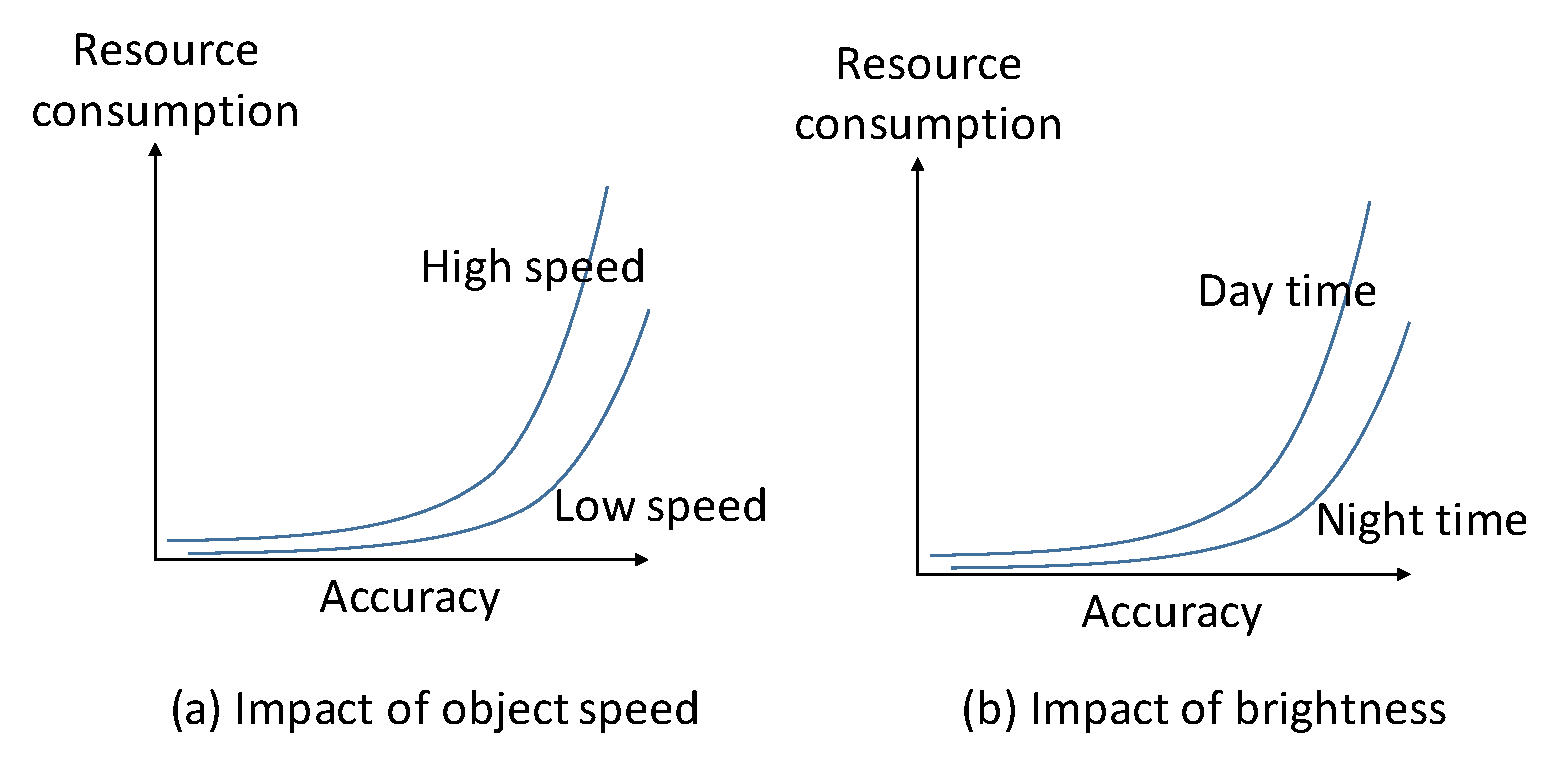
\includegraphics[width=0.45\textwidth]{figures/example.pdf}
\vspace{-0.3cm}
\caption{The resource-accuracy tradeoff varies depending on factors such as object speed, background brightness, etc}
\label{fig:example}
\end{figure}

\subsection{Potentials of adaptive profiling}

Use trace-driven simulation to show the gain of always using the best configuration (with hindsight knowledge).



\subsection{Challenges of adaptive profiling}
\mypara{Strawmen of adapting profiles}
\begin{itemize}
\item what about key frame extraction: profile may not change between two key frames (e.g., constant speed moving objects)
\item what about scene change detection: profile may change even within the same scene (e.g., change of object moving speed).
\end{itemize}

\mypara{Cost of re-profiling}
The takeaway is it is difficult to detect changes of resource-accuracy profile by simply looking at certain ``signal'', thus the need for periodic profiling $\rightarrow$ high cost of exploration cost.

\section{Opportunity of cross-camera profiling}

\subsection{Spatial similarity across cameras}

\section{Design of \name}

\subsection{Cross-camera profiling as a contextual\\multi-armed bandit process}

\subsection{Grouping similar cameras}

\subsection{Amortizing exploration cost}

\subsection{Implementation}

\section{Evaluation}

\section{Related work}


{\scriptsize
\bibliographystyle{abbrv}
\bibliography{}
}

%\appendix

%\input{concerns}

\end{document}


